\section{Optimization model and solution strategy}\label{sec:OptimizationModel}

In this section, the optimization problem is presented. First, the time sequence of decision variables for mFRR is presented. Second, we explain how scenarios for price data are generated for in-sample (IS) training and out-of-sample (OOS) evaluation. Third, we present the compact model formulation. Fourth, we present the two solution strategies for mFRR, including the mFRR bidding policy and scenario decomposition. Finally, we present the full model formulation.

\subsection{Time sequence for decision making}

Figure \ref{fig:timeline_mfrr_variables} shows the stages for making decisions in the mFRR market. First, a reservation bid, $p_{h}^{r,\uparrow}$ is submitted. For any reservation bid accepted, a regulating power bid must be submitted, $\lambda_{h,\omega}^{\text{bid}}$. The reservation and bid are the \textit{first-stage} decisions. The set $\Gamma_{\omega}$, contains all real-time variables in the optimization problem and are the \textit{second-stage} decisions. They control the real-time power, auxillary variables for identifying up- and down-regulation\footnote{Down-regulation refers to the rebound action in this context.}, temperature dynamics, and when to deliver up-regulation according to the bid. For more details, see Section \ref{sec:final_model}. The index, $\omega$, specifies a scenario.


\begin{figure}[!t]\label{fig:timeline_mfrr_variables}
    \centering
    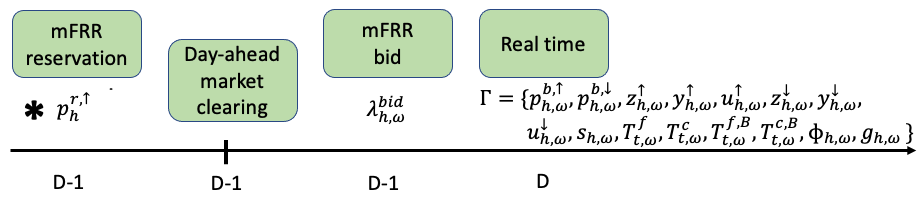
\includegraphics[width=\columnwidth]{../figures/timeline_mfrr_variables.png}
    \caption{Variables related to mFRR up-regulation decisions. The asterisk indicates the first-stage decision.}
\end{figure}

\subsection{Scenario generation}\label{sec:scenario_generation}

To train the optimization model to get a policy for $p_{h}^{r,\uparrow}$ and $\lambda_{h,\omega}^{\text{bid}}$, we generate scenarios for price data using two strategies (where one scenario corresponds to one day):

\begin{enumerate}
    \item Training IS on 2021 price data with varying number of scenarios
    \item Training IS using a lookback of five days
\end{enumerate}

In both cases, balancing prices, $\lambda_{h}^{b}$, are sampled from days where up-regulation happened 1 $\ldots$ 24 hours  with equal probability. In this way, there is emphasis on days and hours where up-regulation happened, and the model should learn a policy taking this into account.

For spot prices, the lookback strategy uses the spot price from the past five days to take advantage of any autocorrelation. The first strategy samples spot price days in 2021. For both strategies, evaluation is done OOS on unseen 2022 price data.

For load shifting, the policy is simply to solve the optimization problem for the next day since the day-ahead market clearing happens in advance.

\subsection{Compact model formulation}

The compact model formulation is presented in Problem \ref{P1:compact_model}. The objective function is the sum of the revenue from the reservation bid, i.e., first-stage decisions, and the \textit{expected} revenue and costs from the regulating power bid and subsequent rebound and penalties. Constraint (\ref{P1:eq2}) incorporates activation of the bid, and constraint (\ref{P1:eq3}) incorporates the temperature dynamics in the freezer.


\begin{subequations}\label{P1:compact_model}
    \begin{align}
        \underset{\bm{p}^{r,\uparrow}, \bm{\lambda}_{\omega}^{\text{bid}}, \bm{\Gamma}_{\omega}}{\textrm{max}} \quad & f(\bm{p}^{r,\uparrow}) + \sum_{\omega} \pi_{\omega} g(\bm{\Gamma}_{\omega}) \label{P1:eq1}
        \\
        s.t \quad                                                                                                    & h(\bm{p}^{r,\uparrow}, \bm{\lambda}_{omega}^{\text{bid}}, \bm{\Gamma}_{\omega}) \leq 0, \quad \forall{\omega}\label{P1:eq2}                                                                     \\
        \quad                                                                                                        & \text{State-space model in } (\ref{eq:2ndFreezerStateSpace}), \quad \forall{\omega} \label{P1:eq3}
        \\
        \quad                                                                                                        & \Bigl( \bm{p}^{r,\uparrow}, \bm{\lambda}_{\omega}^{\text{bid}}, \bm{p}_{\omega}^{b,\uparrow}, \bm{p}_{\omega}^{b,\downarrow}, \bm{s}_{\omega}, \bm{T}_{\omega}^{c}, \bm{T}_{\omega}^{f}, \notag \\ \quad & \quad \bm{T}_{\omega}^{c, B}, \bm{T}_{\omega}^{f,B}, \bm{\phi}_{\omega}, \bm{g}_{\omega} \Bigr) \in \mathbb{R}^{n}  \label{P1:eq4}
        \\
        \quad                                                                                                        & \bm{u}_{\omega}, \bm{z}_{\omega}, \bm{y}_{\omega} \in \{0,1\}  \label{P1:eq5}
    \end{align}
\end{subequations}

For mFRR, the objective function in (\ref{eq:mFRRObjective}) corresponds to $f$ and $g$ in (\ref{P1:eq1}). For load shifting, the optimization problem is simply obtained by removing bid constraints and replacing the (\ref{P1:eq1}) with (\ref{eq:LoadShiftingObjective}), and then solving the optimization problem for the next day.


\subsection{Solution strategy}\label{sec:solution_strategy}

To solve Problem (\ref{P1:compact_model}), we first need to specify a bidding policy that can readily be used OOS. We do so by choosing an affine bidding policy. It is then shown how the bidding policy is implemented using McCormick relaxation. Finally, it shown how to solve (\ref{P1:compact_model}) for many scenarios using decomposition.

\subsubsection{Affine bidding policy}

A bidding policy needs to be easy to follow OOS for the trader. We choose an affine bidding policy, i.e., a linear function of the spot price. The bidding policy is given by:

\begin{subequations}\label{eq:affine_policy}
    \begin{align}
        \lambda^{bid}_{h,\omega} & = \alpha \lambda_{h,\omega}^{s,\text{diff}} + \beta + \lambda_{h,\omega}^{s}, \quad \forall{\omega}, \forall{h} \in \{1\ldots23\}\label{affine_policy:1} \\
        \alpha                   & \geq 0\label{affine_policy:2}                                                                                                                            \\
        \beta                    & \geq 0\label{affine_policy:3}
    \end{align}
\end{subequations}

Here, the idea in (\ref{eq:affine_policy}) is that the spot price differential approximates a reasonable policy since a large price differential in hour $h$ means that the spot price at time $h+1$ is much higher. Hence, a large bid at time $h$ is desirable such that the probability of being activated in hour $h$ and rebounding in an expensive hour $h+1$ is low (cf. Section \ref{sec:mFRR}).

Variables $\alpha$ and $\beta$ is then learned IS and fixed for OOS evaluation. After the day-ahead market clearing, (\ref{eq:affine_policy}) can easily be used to specify bids for the next day, i.e., $\lambda_{h,\omega}^{\text{bid}}$.

\subsubsection{McCormick relaxation}\label{sec:mccormick}

As explained in Section \ref{sec:mFRR}, activation of mFRR reservation only happens when certain price conditions are met. This is formalized in the following constraint:

\begin{equation}\label{eq:bid_constraint}
    p^{b, \uparrow}_{h,\omega} + s_{h,\omega} \geq p^{r,\uparrow}_{h} \cdot \mathbbm{1}_{h,\omega}^{(\lambda^{bid}_{h} < \lambda^{b}_{h,\omega}, \lambda^{b}_{h,\omega} > \lambda^{s}_{h})}, \quad \forall{h,\omega}
\end{equation}

Eq. (\ref{eq:bid_constraint}) says that the real-time up-regulation plus a slack variable must be greater than or equal to the reservation if the bid is lower than the balancing price and if up-regulation is needed in hour $h$. It is a bi-linear constraint so McCormick relaxation is used to convert (\ref{eq:bid_constraint}) to a linear constraint by introducing auxillary variables, $\phi_{h,\omega}$ and $g_{h,\omega}$:

\begin{subequations}\label{eq:bid_constraint_relaxed}
    \begin{align}
        \lambda_{h,\omega}^{b} - \lambda_{h}^{s} \geq \lambda_{h,\omega}^{bid} - M \cdot (1 - g_{h,\omega}) , \quad                                   & \forall{h,\omega}             \label{con_bid:subeq1} \\
        \lambda_{h,\omega}^{bid} \geq \lambda_{h,\omega}^{b} - \lambda_{h}^{s} - M \cdot (1 - g_{h,\omega}) , \quad                                   & \forall{h,\omega}             \label{con_bid:subeq2} \\
        p^{b, \uparrow}_{h,\omega} \leq \phi_{h,\omega} \cdot \mathbbm{1}_{h,\omega}^{\lambda^{b}_{h,\omega} > \lambda^{s}_{h}}, \quad                & \forall{{h,\omega}}           \label{con_bid:subeq3} \\
        p^{b, \uparrow}_{h,\omega} + s_{h,\omega} \geq \phi_{h,\omega} \cdot \mathbbm{1}_{h,\omega}^{\lambda^{b}_{h,\omega} > \lambda^{s}_{h}}, \quad & \forall{{h,\omega}}           \label{con_bid:subeq4} \\
        -g_{h,\omega} \cdot M \leq \phi_{h,\omega}, \quad                                                                                             & \forall{h,\omega}             \label{con_bid:subeq5} \\
        \phi_{h,\omega} \leq g_{h,\omega} \cdot M, \quad                                                                                              & \forall{h,\omega}             \label{con_bid:subeq6} \\
        -(1 - g_{h,\omega}) \cdot M \leq \phi_{h,\omega} - p^{r,\uparrow}_{h}, \quad                                                                  & \forall{h,\omega}             \label{con_bid:subeq7} \\
        \phi_{h,\omega} - p^{r,\uparrow}_{h} \leq (1 - g_{h,\omega}) \cdot M, \quad                                                                   & \forall{h,\omega}             \label{con_bid:subeq8}
        % \lambda_{h,\omega}^{bid} \leq \lambda^{Max} \label{con_bid:subeq9}
    \end{align}
\end{subequations}

Constraints (\ref{con_bid:subeq1}-\ref{con_bid:subeq2}) ensures that $g_{h,\omega} = 1$ when the balancing price minus the spot price is larger than our bid, $\lambda^{bid}_{h}$, and zero otherwise. Constraints (\ref{con_bid:subeq3}-\ref{con_bid:subeq4}) sets the TCL up-regulation equal to $\phi_{h,\omega}$ (or incurs a penalty) if there is an up-regulation event in the system, i.e., if $\mathbbm{1}_{h,\omega}^{\lambda^{b}_{h,\omega} > \lambda^{s}_{h}} = 1$. Constraints (\ref{con_bid:subeq5}-\ref{con_bid:subeq6}) ensures that $\phi_{h,\omega} = 0$ when $g_{h,\omega} = 0$, i.e., when the balancing price differential is smaller than our bid. Constraints (\ref{con_bid:subeq7}-\ref{con_bid:subeq8}) ensures that $\phi_{h,\omega}$ is equal to the reservation capacity, $p^{r,\uparrow}_{h}$, whenever $g_{h,\omega} = 1$, i.e., whenever the bid is smaller than the balancing price differential.

\subsubsection{Scenario decomposition with ADMM}

When solving Problem (\ref{P1:compact_model}) with many scenarios, it quickly becomes computationally intractable due to the number of binaries and intertemporal constraints. To solve it, the Alternating Direction Method of Multipliers (ADMM) algorithm is used which is a decomposition method that solves a large-scale optimization problem by decomposing it into smaller subproblems \cite{boyd2011distributed}. In (\ref{P1:compact_model}), each scenario is solved as a subproblem by setting:

\begin{equation}\label{eq:non_anticipativity}
    \bm{p}^{r,\uparrow} \rightarrow \bm{p}^{r,\uparrow}_{\omega}, \quad \alpha \rightarrow \alpha_{\omega}, \quad \beta \rightarrow \beta_{\omega}
\end{equation}

The ADMM algorithm will converge by achieving consensus on first- and second-stage stage decisions, but it is only a heuristic for MILPs \cite{hong2016convergence}.

\subsection{Final model formulation}\label{sec:final_model}

% Describe objective function for mFRR and load shifting.

% The set, $\Psi$, then contains all the optimization variables:

% \begin{align}\label{set:OptVariables}
%     \Psi = \{p_{h,\omega}, p^{r, \uparrow}_{h}, & s_{h,\omega}, p^{b, \uparrow}_{h,\omega}, p^{b, \downarrow}_{h,\omega}, u^{\uparrow}_{h,\omega}, y^{\uparrow}_{h,\omega}, z^{\uparrow}_{h,\omega}, u^{\downarrow}_{h,\omega}, y^{\downarrow}_{h,\omega}, z^{\downarrow}_{h,\omega}, \notag \\ & T^{f}_{\omega, t}, T^{c}_{\omega, t}, T^{f,B}_{t}, T^{c, B}_{t}, \lambda_{h}^{bid}, \phi_{h,\omega}, g_{h,\omega}, \Delta \}
% \end{align}

The final optimization model is a two-stage stochastic MILP and is described in full detail in this subsection. First, all auxillary variables and constraints are presented. Second, constraints related to the power consumption for the freezer is shown. Third, the physical constraints for the temperatures are presented. Lastly, the rebound constraints are presented.


\subsubsection{Auxillary variables and constraints}\label{sec:aux_constraints}

First, we describe the necessary auxillary variables and constraints to identify when up- and down-regulation occurs compared to the baseline power, $P^{\text{Base}}_{h}$. This is required since the costs and revenues from up-regulation and rebound must be determined explicitly. We therefore introduce the following six binary variables \cite{morales2013integrating}:
\\
\begin{itemize}
    \item $u^{\uparrow}_{h,\omega} \in \{0,1\}$ equal to 1 when starting to deliver up-regulation
    \item $y^{\uparrow}_{h,\omega} \in \{0,1\}$ equal to 1 during up-regulation
    \item $z^{\uparrow}_{h,\omega} \in \{0,1\}$ equal to 1 when to stopping up-regulation
    \item $u^{\downarrow}_{h,\omega} \in \{0,1\}$ equal to 1 when starting to deliver down-regulation
    \item $y^{\downarrow}_{h,\omega} \in \{0,1\}$ equal to 1 during down-regulation
    \item $z^{\downarrow}_{h,\omega} \in \{0,1\}$ equal to 1 when to stopping down-regulation
\end{itemize}

\noindent The following constraints implements the logic:

\begin{subequations}\label{eq:auxillary_constraints}
    \begin{align}
        u_{h-1,\omega}^{\uparrow} - u_{h,\omega}^{\uparrow} + y_{h,\omega}^{\uparrow} - z_{h,\omega}^{\uparrow} = 0 \quad         & \forall{\omega}, \forall{h} = \{2 \ldots 24 \} \\
        y_{h,\omega}^{\uparrow} + z_{h,\omega}^{\uparrow} \leq 1 \quad                                                            & \forall{h,\omega}                              \\
        u_{h-1,\omega}^{\downarrow} - u_{h,\omega}^{\downarrow} + y_{h,\omega}^{\downarrow} - z_{h,\omega}^{\downarrow} = 0 \quad & \forall{\omega}, \forall{h} = \{2 \ldots 24 \} \\
        y_{h,\omega}^{\downarrow} + z_{h,\omega}^{\downarrow} \leq 1 \quad                                                        & \forall{h,\omega}                              \\
        u_{h,\omega}^{\uparrow} + u_{h,\omega}^{\downarrow} \leq 1 \quad                                                          & \forall{h,\omega}                              \\
        y_{h,\omega}^{\uparrow} + y_{h,\omega}^{\downarrow} \leq 1 \quad                                                          & \forall{h,\omega}                              \\
        z_{h,\omega}^{\uparrow} + z_{h,\omega}^{\downarrow} \leq 1 \quad                                                          & \forall{h,\omega}
    \end{align}
\end{subequations}

\subsubsection{Power constraints}\label{sec:power_constraints}

The power consumption of the freezer is constrained by:

\begin{subequations}\label{eq:power_constraints}
    \begin{align}
        p_{h,\omega} = P^{\text{Base}}_{h} - p^{b, \uparrow}_{h,\omega} + p^{b, \downarrow}_{h,\omega}, \quad                                                                                          & \forall{h,\omega}                                                                             \label{con_power:subeq1}  \\
        p^{r, \uparrow}_h \leq P^{\text{Base}}_h, \quad                                                                                                                                                & \forall{h}                                                                                     \label{con_power:subeq2} \\
        p^{b, \uparrow}_{h,\omega} \leq p^{r, \uparrow}_h \mathbbm{1}_{h,\omega}^{\lambda^{b}_{h,\omega} > \lambda^{s}_{h}} , \quad                                                                    & \forall{h,\omega}                                                                             \label{con_power:subeq3}  \\
        p^{b, \uparrow}_{h,\omega} \leq u_{h,\omega}^{\uparrow} (P^{\text{Base}}_{h} - P^{Min}) , \quad                                                                                                & \forall{h,\omega}                                                                             \label{con_power:subeq4}  \\
        p^{b, \downarrow}_{h,\omega} \leq u^{\downarrow}_{h,\omega} (P^{\text{Nom}} -P^{\text{Base}}_{h}), \quad                                                                                       & \forall{h,\omega}                                                                             \label{con_power:subeq5}  \\
        P^{Min} \leq p_{h,\omega} \leq P^{\text{Nom}}, \quad                                                                                                                                           & \forall{h,\omega}                                                                             \label{con_power:subeq6}  \\
        0 \leq s_{h,\omega} \leq P^{\text{Base}}_{h}, \quad                                                                                                                                            & \forall{h,\omega}                                                                             \label{con_power:subeq7}  \\
        p^{b, \uparrow}_{h,\omega} + s_{h,\omega} \geq p^{r,\uparrow}_{h} \cdot \mathbbm{1}_{h,\omega}^{(\lambda^{bid}_{h} < \lambda^{b}_{h,\omega}, \lambda^{b}_{h,\omega} > \lambda^{s}_{h})}, \quad & \forall{h,\omega} \label{con_power:subeq8}                                                                              \\
        p^{b, \downarrow}_{h,\omega} \geq 0.10 \cdot u^{\downarrow}_{h,\omega} (P^{\text{Nom}} - P^{\text{Base}}_{h}), \quad                                                                           & \forall{h,\omega}                                                                             \label{con_power:subeq9}  \\
        p^{r, \uparrow}_{h} \leq P^{\text{Base}}_{h} (1 - \mathbbm{1}_{h}^{df}), \quad                                                                                                                 & \forall{h} \label{con_power:subeq10}
    \end{align}
\end{subequations}

Constraint (\ref{con_power:subeq1}) sets the power equal to the baseline power unless there is up- or down-regulation. Constraint (\ref{con_power:subeq2}) bounds the reservation power to the baseline power. Constraint (\ref{con_power:subeq3}) ensures that up-regulation is zero when the system does not need it, and at the same time bounds it to the reservation power. Constraint (\ref{con_power:subeq4}) ensures that up-regulation is 0 whenever $u^{\uparrow}_{h,\omega} = 0$, and otherwise bounded to the maximum power that can be upregulated. Constraint (\ref{con_power:subeq5}) works the same way for down-regulation. Constraint (\ref{con_power:subeq6}) bounds the power to be between the minimum and nominal power. Constraint (\ref{con_power:subeq7}) bounds the slack variable which is the energy not delivered as promised. Constraint (\ref{con_power:subeq8}) is the bi-linear constraint from (\ref{eq:bid_constraint}). Constraint (\ref{con_power:subeq9}) ensures that down-regulation is equal to at least 10\% of the down-regulation capacity. Lastly, constraint (\ref{con_power:subeq10}) prohibits any up-regulation when defrosting occurs.

\subsubsection{Physical constraints}\label{sec:temperature_constraints}

The state-space model in (\ref{eq:2ndFreezerStateSpace}) is simply added as constraints with $p_{t,\omega}$ being the power of the freezer and an additional index for each scenario, $\omega$.

Note, the freezer specific variables are indexed by $t$, representing a time step $dt = 0.25$ whereas all other variables are indexed by hour $h$.

Furthermore, there is a set of identical constraints to (\ref{eq:2ndFreezerStateSpace}) that simulates the baseline temperatures, $T^{f,B}_{t}$ and $T^{c,B}_{t}$, using the baseline power, $P^{Base}_{h}$. These are used for the following boundary constraint, as well as the rebound constraints in Section \ref{sec:rebound_constraints}.

\begin{align}\label{eq:boundary_constraint}
    T^{f}_{96,\omega} \leq T^{f, \text{Base}}_{96}, \quad \forall{\omega}
\end{align}

The boundary constraint in (\ref{eq:boundary_constraint}) ensures that the optimization does not exploit the end state.

Temperature constraints to the air temperature can easily be added to limit the flexibility of the TCL by introducing a maximum temperature difference to the baseline temperature, $\Delta^{\text{max}}$:

\begin{subequations}\label{eq:delta_max_constraints}
    \begin{align}
        T^{c,\text{Base}}_{t} - \Delta \leq T^{c}_{t, \omega}, \quad & \forall{t, \omega} \\
        T^{c,\text{Base}}_{t} - \Delta \geq T^{c}_{t, \omega}, \quad & \forall{t, \omega} \\
        \Delta \leq \Delta^{\text{max}}
    \end{align}
\end{subequations}

\subsubsection{Rebound constraints}\label{sec:rebound_constraints}

The rebound constraints ensures that a rebound happens right after an up-regulation by down-regulating:

\begin{subequations}\label{eq:rebound_constraints_1}
    \begin{align}
        y^{\downarrow}_{h, \omega} \geq z^{\uparrow}_{h, \omega}, \quad & \forall{h, \omega} \\
        y^{\downarrow}_{h, \omega} \leq z^{\uparrow}_{h, \omega}, \quad & \forall{h, \omega}
    \end{align}
\end{subequations}


Furthermore, the following rebound constraints ensures that the rebound will take place until the food temperature is equal to the baseline food temperature, which can be considered the setpoint food temperature:

\begin{subequations}\label{eq:rebound_constraints_2}
    \begin{align}
        \sum_{t=4\cdot(h-1)}^{4 h} T^{f}_{t, \omega} - T^{f, \text{Base}}_{t} \geq - (1 - z^{\downarrow}_{h, \omega}) \cdot M, \quad & \forall{\omega}, \forall{h} \\
        \sum_{t=4\cdot(h-1)}^{4 h} T^{f}_{t, \omega} - T^{f, \text{Base}}_{t} \leq - (1 - z^{\downarrow}_{h, \omega}) \cdot M, \quad & \forall{\omega}, \forall{h}
    \end{align}
\end{subequations}

In constraints (\ref{eq:rebound_constraints_2}), $M$ is a sufficiently big number such that the food temperature is allowed to deviate from the baseline.

Lastly, the following constraint ensures that up-regulation happens before down-regulation:

\begin{align}\label{eq:up_regulation_first}
    \sum_{k=0}^{h} y^{\downarrow}_{\omega, k} \leq y^{\uparrow}_{\omega, k}, \quad \forall{h, \omega}
\end{align}

This makes sense since it is not possible (or at least difficult) to anticipate potential up-regulation events in the power grid. As such, it does not make sense to pre-cool (or pre-heat) a TCL in the context of mFRR.
